% \author{22371027-汤睿璟}
% 设置页面边距(word标准页面)
\documentclass[a4paper]{article}
\usepackage{cite} % 加在文章最开头,表示你这篇文章要引用别的东西。
\usepackage{geometry}
\geometry{a4paper,left=2.7cm,right=2.7cm,top=2.54cm,bottom=2.54cm}
\usepackage{tikz}
\usetikzlibrary{shapes.geometric, arrows}
\usepackage{wrapfig}


%导入ctex包
\usepackage[UTF8,heading=true]{ctex}
\tikzset{
	startstop/.style={
		rectangle,
		rounded corners,
		minimum width=3cm,
		minimum height=1cm,
		text centered,
		draw=black,
		fill=red!30
	},
	io/.style={
		trapezium,
		trapezium left angle=70,
		trapezium right angle=110,
		minimum width=3cm,
		minimum height=1cm,
		text centered,
		draw=black,
		fill=blue!30
	},
	process/.style={
		rectangle,
		minimum width=3cm,
		minimum height=1cm,
		text centered,
		draw=black,
		fill=orange!30
	},
	decision/.style={
		diamond,
		aspect=2, % 控制菱形的宽高比
		minimum width=3cm,
		minimum height=1cm,
		text centered,
		draw=black,
		fill=green!30
	},
	arrow/.style={
		thick,
		-Stealth % 使用Stealth箭头样式
	}
}

%设置摘要格式
\usepackage{abstract}
\setlength{\abstitleskip}{0em}
\setlength{\absleftindent}{0pt}
\setlength{\absrightindent}{0pt}
\setlength{\absparsep}{0em}
\renewcommand{\abstractname}{\textbf{\zihao{4}{摘要}}}
\renewcommand{\abstracttextfont}{\zihao{-4}} %设置摘要正文字号

%设置页眉和页脚,只显示页脚居中页码
\usepackage{fancyhdr}
\pagestyle{plain}

%调用数学公式包
\usepackage{amssymb}
\usepackage{amsmath}

%调用浮动包
\usepackage{float}
\usepackage{subfig}
% \captionsetup[figure]{labelsep=space} %去除图标题的冒号
% \captionsetup[table]{labelsep=space} %去除表格标题的冒号
%设置标题格式
\ctexset {
	%设置一级标题的格式
	section = {
		name={,、},
		number=\chinese{section}, %设置中文版的标题
		aftername=,
	},
	%设置三级标题的格式
	subsubsection = {
		format += \zihao{-4} % 设置三级标题的字号
	}
}


%使得英文字体都为Time NewTown
%\usepackage{times}

%图片包导入
\usepackage{graphicx}
\graphicspath{{figures/}} %图片在当前目录下的figures目录

%参考文献包引入
\usepackage{cite}
\usepackage[numbers,sort&compress]{natbib}

%代码格式
\usepackage{listings}
\usepackage{graphicx}%写入python代码
\usepackage{pythonhighlight}%python代码高亮显示
\lstset{
	%numbers=left, %设置行号位置
	%	numberstyle=\tiny, %设置行号大小
	keywordstyle=\color{blue}, %设置关键字颜色
	commentstyle=\color[cmyk]{1,0,1,0}, %设置注释颜色
	escapeinside=``, %逃逸字符(1左面的键),用于显示中文
	breaklines, %自动折行
	extendedchars=false, %解决代码跨页时,章节标题,页眉等汉字不显示的问题
	xleftmargin=1em,xrightmargin=1em, aboveskip=1em, %设置边距
	tabsize=4, %设置tab空格数
	showspaces=false %不显示空格
}


\renewcommand{\refname}{}

%item包
\usepackage{enumitem}

%表格加粗
\usepackage{booktabs}

%设置表格间距
\usepackage{caption}

%允许表格长跨页
\usepackage{longtable}

%伪代码用到的宏包
\usepackage{algorithm}
\usepackage{algpseudocode}

\usepackage{accents}

\title{编译实验 - 设计报告}
\date{}

\begin{document}
	\maketitle
	\vspace{-6em} %设置摘要与标题的间距
	\zihao{-4} %设置正文字号
	
	\begin{center}22371027-汤睿璟\end{center}
	% \author{22371027-汤睿璟}
	
	\section{参考编译器设计}
	
	编译器主要参考了 Wokron 学长为编译课设计的实例编译器 tolangc。
	
		\subsection{tolangc}
		
		tolangc 的前端在 libs/tolang 文件夹下,主要由 $lexer$, $parser$, $AST$ 和 $visiter$ 四个部分构成,分别处理词法分析、语法分析、抽构建象语法树和中间代码生成四项任务。
		其符号表由 $libs/tolang/include/symtable.h$ 文件中 SymbolTable 类来统一管理。
		前端的错误处理则由 同目录下的 error.h 文件下的 ErrorReporter 完成错误的记录和输出。
	
	\section{编译器总体设计}
	
		本人设计的编译器由前端和后端构成,前端包括词法分析、语法分析、符号表构建和管理、抽象语法树构建和中间代码生成。\textbf{后端的相关内容随实验和理论课推进后进行补充。}
		
		\subsection{文件结构}
		
			前端的文件结构为:
			
			\begin{algorithm}[H]
				libs/tang \\
				├── Ast.cpp \\
				├── Ast.hpp: 存放 AST 有关的类的定义,每个类表示一个语法成分 \\
				├── ErrorReporter.cpp \\
				├── ErrorReporter.hpp: 错误处理程序,主要功能为收集错误并输出 \\
				├── Evaluate.cpp: $Visitor$ 类的有关求常量表达式的值的方法 \\
				├── LLVMVisitor.cpp: $Visitor$ 类的有关生成 $llvm$ 的方法 \\
				├── Lexer.cpp \\
				├── Lexer.hpp: 词法分析器 \\
				├── LoopStack.hpp: 循环栈,用于存放每一层循环的信息如基本块划分等 \\
				├── Parser1.cpp \\
				├── Parser1.hpp: 语法分析器,用于生成 AST \\
				├── Symbol.cpp \\
				├── Symbol.hpp: 符号类型、符号、符号表的相关定义 \\
				├── Token.cpp \\
				├── Token.hpp: Token 及其类型的定义,主要供词法分析器使用 \\
				├── Visitor.cpp \\
				├── Visitor.hpp: 语义分析和代码生成器
			\end{algorithm}
			
			中间代码的文件结构如下,具体解释见代码生成
			
			\begin{algorithm}[H]
				libs/llvm
				└── IR
				├── Argument.cpp \\
				├── Argument.hpp: Argument 类型的 $Value$ 定义 \\
				├── BasicBlock.cpp \\
				├── BasicBlock.hpp: 基本块有关的的定义 \\
				├── Common.hpp: Forward Declaration 以及一些都要用到的头文件 \\
				├── Constant.cpp \\
				├── Constant.hpp: $llvm$ 的 constant 类型的 value(抽象类) \\
				├── ConstantData.cpp \\
				├── ConstantData.hpp: $llvm$ 的 ConstantData 类型的 value(抽象类 \\
				├── Function.cpp \\
				├── Function.hpp: $Function$ 类型 \\
				├── GlobalString.cpp \\
				├── GlobalString.hpp: 不记得 $llvm$ 有没有这个类型了,表示全局字符串,继承自 GlobalValue \\
				├── GlobalValue.cpp \\
				├── GlobalValue.hpp: GlobalValue 类型,其下主要有全局变量和字符串常量继承自它。 \\
				├── GlobalVariable.cpp \\
				├── GlobalVariable.hpp: 全局变量 \\
				├── IRPrinter.hpp: 用于打印生成的中间代码 \\
				├── Instructions.cpp \\
				├── Instructions.hpp: $llvm$ 的基本指令 \\
				├── LLVMContext.cpp \\
				├── LLVMContext.hpp: llvmContext 类,主要用于存放一些常用的对象。 \\
				├── Module.cpp \\
				├── Module.hpp: $llvm$ 顶层模块,下有众多静态存储量和众多 $Function$ \\
				├── Type.cpp \\
				├── Type.hpp: $llvm$ 的类型体系 \\
				├── Use.cpp \\
				├── Use.hpp: llvm-IR 中规定的 User 与 $Value$ 间的 use 关系 \\
				├── User.cpp \\
				├── User.hpp: $llvm$ 的 User 类型,继承自 $Value$ \\
				├── Value.cpp \\
				└── Value.hpp: $Value$ 类型
			\end{algorithm}
		
		\subsection{编译流程}
		
			该编译器主要的编译流程如下图所示
			
			\begin{figure}[H]
				\centering
				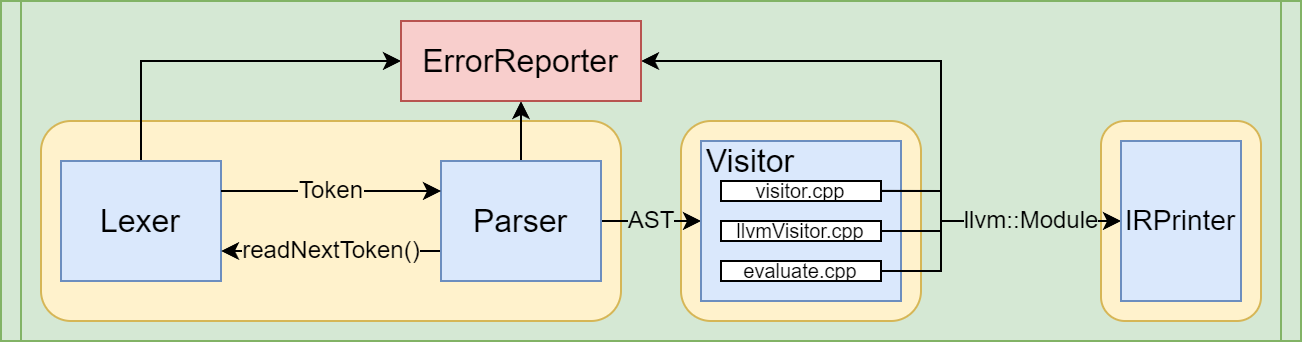
\includegraphics[width=0.9\linewidth]{images/proc.png}
				\caption{编译流程}
				\label{fig:label4}	
			\end{figure}
			
			其中由于没有考虑生成机器相关代码,$Visitor$ 生成出来的中间代码直接传递到了 IRPrinter。
	
	\section{词法分析设计}
	
		词法分析器通过一遍完成文件的读入,并将输入的原文件在对外接口中暴露为 $Token$ 流。 
		在编码前,原本预计使用 vector<Token> 将所有读入的 $Token$ 进行保存,再进行处理。后续发现这种处理方式会带来额外的内存开支,并在随后废弃了这种想法。
		
		Lexer 在 $Lex$ 标识符时会对关键字进行检查,并对错误的关键字进行相应的错误处理。对于读取到并且处理好的关键字,可以通过调用 $Lexer$ 的 nextToken() 接口中读取到 $Lex$ 到的下一个 Token。该编译器除了读取课程组给定的字符以外,同时新增了 EOF、Comment 以及非法字符三种不同的 $Token$ 类型。
		
        为了能够同时让词法分析和语法分析能够同时进行,Lexer 不会一次性读取完 nextToken(),而是当 $Parser$ 调用 nextToken() 函数的时候才会对下一个字符进行解析。
	
	\section{语法分析设计}

		Parser 本质上是一个自顶向下的语法分析器。他通过不断读取 $Lexer$ 的单词,根据语法规则构建语法树。
		
		\subsection{第一次设计:回溯}
		
			在最初的设计中,由于语法分析相关理论的缺失,本人企图设计一回溯的编译器。这也是文件结构中有关 $Parser$ 的文件不叫 Parser.hpp 而是 Parser1.hpp 的原因,即第一次设计的语法分析器因为回溯而被抛弃。
			
			个人认为回溯带来的最大问题在于将需要将读取到的 $Token$ 返回给 Lexer,这意味着每次 parse 的时候,Parser 和 $Lexer$ 两边都需要有一个关于 $Token$ 的有序表来记录获取到的 Token。这一点不仅增加了设计的复杂性,而且增加时间和空间开销,因此在重构代码时被舍弃。
        
        \subsection{左递归文法}

        	课程组提供的 SysY 语言的文法定义中,部分有关 AddExp、MulExp 等非终结符的推导规则存在直接左递归。为此,编译器通过适当修改文法,既保证了输出的正确性,同时避免左递归的问题。
        
        \subsection{Statement 的处理}
        
	        尽管 SysY 的文法的规则在多数情况下为 LL(1) 文法,即可以通过查看 $Lexer$ 得到的下一个字符,并将其与 FOLLOW 集或者不同候选式的 FIRST 集进行比较来确定用于递归下降的规则。但是在对于 Statement 候选式的判断中,不论往后查看多少字符,都存在反例使得无法确定非终结符的候选式,也就是说 SysY 实际上不是 LL 文法。
	        
	        在 Statement 语法成分中,当接下来的输入为一数组元素的 $LVal$ 的时候,由于索引为一 Exp,因此无法通过查看 $Lexer$ 顶端的字符来判断该左值之后是赋值语句、$getint$ 还是 $getchar$ 语句。
	        
	        对此,编译器在尝试确定往其余候选式之后如果发现无法通过查看下面的字符来确定候选式的话,就会将数组元素这一 $LVal$ 提取出来,作为不同候选式的公共前缀。在此处,提取出的公共前缀即为 $LVal$ 这一语法成分。在 parse 完 $LVal$ 后即可比较读入的字符确定候选式,并将提取出来的前缀通过继承属性传递给下层语法成分的 $Parser$ 过程来决定是哪一个语法成分。
        	
        对于每一个非终结符,编译器使用了一指针/指针数组指向其子节点,表明该语法成分可以推导出的语法成分。实现采用了 $unique\_ptr$ 来完成,因为语法成分只需要存在于语法树中,而不需要作为其他对象的属性出现。这也是参考 tolangc 而设计的。
			
	\section{语义分析设计}
		
		语义分析主要完成剩余错误处理、符号表构建和 $llvm$ 中间代码生成的工作。llvm 生成的部分将放在下一个 section 中进行讲解。
		
		\subsection{符号表构建}
		
			语义分析最重要的就是符号表管理。尽管现在工业上有更为复杂的方式去实现符号表的管理,本人设计的编译器还是使用了简单实用的栈式符号表。在编译原理课程中,我们接触的符号表主要是基于分程序结构而构建的符号表,因此里面的特定分类是不必要的,比如说特别区分 type 和 kind。SysY 作为 C 语言的子集(至少大部分是包含在 C 语言的规范中的),也应当遵循 C 语言的设计理念,而 C 语言的设计理念就是一般化。因此所有进栈的符号,不论是不可修改类型还是函数类型,均所谓一个 $Symbol$ 压入符号表中,并记录其所在的作用域层次。
			
			栈式符号表虽然简单,但是在运行完语义分析后却不会保留下来任何符号信息。但是语义分析的评测程序,由于符号表的输出顺序是根据作用域的开始次序而非结束次序来进行的,因此需要再建立一个全局符号表来存储用于评测的符号表。该符号表会在正常使用时关闭。当然,在构建和查找符号表的时候还需要进行标识符相关的错误处理。
			
		\subsection{符号类型}
		
			Symbol.hpp 文件主要定义了符号类型、符号以及符号表三个类。其中最为核心的当属符号类型。
			
			C 语言的符号类型更加地一般化,但是 SysY 语言定义的符号类型相比之下并没有那么多的约束,因此此处为了简单起见,将类型分为了几类:
			
			\begin{enumerate}
				\item Int
				\item Char
				\item Void
				\item IntArray
				\item CharArray
				\item Function
			\end{enumerate}
			
			此外:基本类型与数组类型均携带一个 $const$ 标记,表明这个数据类型是不是一个不可修改类型。$function$ 类允许查看参数类型和返回值类型。$SymbolType$ 类重载了相等和不相等的运算符,用于符号之间进行类型比较。
		
	\section{代码生成设计}
	
		本编译器采用了 llvm-IR 作为生成的中间代码。生成 $llvm$ 方面和构建符号表同步进行,以提高生成中间代码的效率,即在 Visit 的同时生成 llvm-IR。
		
		llvm 的所有组成部分写成了一个单独的 $llvm$ 库,并在 $Visitor$ 中调用库函数进行中间代码生成。
		
		在具体代码方面,llvm 的主要架构继承自 llvm-project 中关于 llvm-IR 的设计架构。llvm-project 中的内容非常多,该编译器中只对其中的几个类完成了简单的实现。中间代码的整体逻辑结构如下:
		
		\begin{figure}[H]
		 	\centering
		 	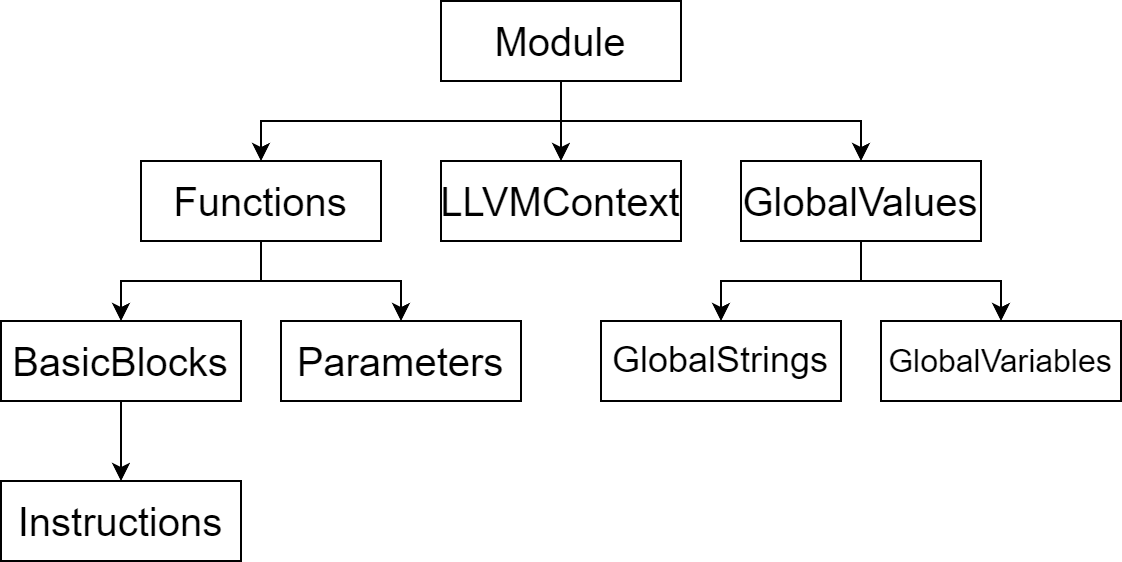
\includegraphics[width=0.7\linewidth]{images/structure.png}
		 	\caption{逻辑结构}
		 	\label{fig:label6}	
		\end{figure}
		
		实现的主要 $Value$ 类型有:
		
		\begin{figure}[H]
			\centering
			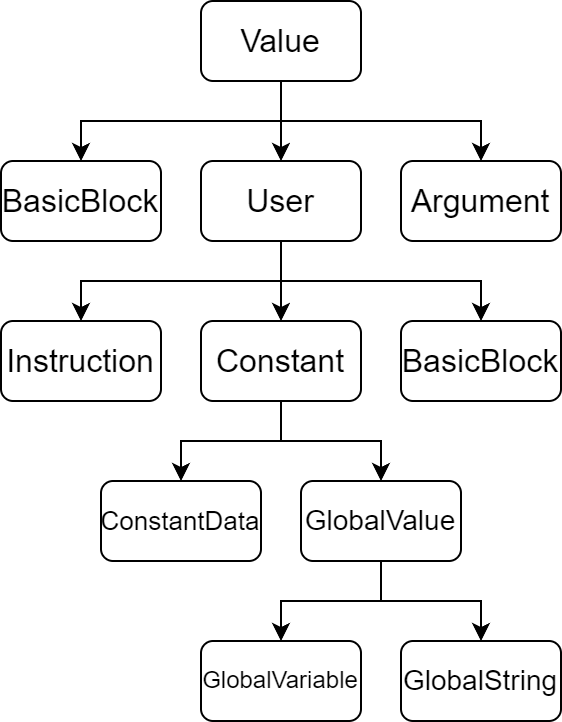
\includegraphics[width=0.5\linewidth]{images/inheritate.png}
			\caption{继承关系}
			\label{fig:label5}	
		\end{figure}
				
		此外,编译器继承了 llvm-IR 的使用关系,即通过 user-usee 构建 User 与 $Value$ 的使用关系,以便于后续进行代码优化。
		
		编译器继承了 llvm-IR 关于变量类型的设计思想,并对整数、数组、指针、$void$ 等类型类型提供了简单的实现。
		
		下面说一些具体实现。
		
		\subsection{$Visitor$ 生成 llvm-IR 流程}
		
			$Visitor$ 类中包含 $\_curModule$、$\_curFunction$、$\_curBlock$ 三个成员属性,表示当前所处的 $llvm$ 模块、函数和基本块分别是哪个。每一个成员属性大都是指向目标的指针,因此可以通过成员属性方便地找到插入指令的位置。
		
		\subsection{for 语句实现}
		
			每当遇到一个 $for$ 循环时,将初始条件与先前的基本块合并,并新创建四个 BasicBlock,分别表示循环判断条件、循环体、更新条件和循环外的基本块。按照四个基本块所对应的 AST 部分进行翻译即可。
			
			此外,当遇到 $break$ 指令和 $continue$ 指令的时候,需要新建跳转到目标代码的跳转指令,同时新建一个基本块表示这条跳转指令后面跟着的指令。当然,这些指令实际上并不会被运行,可以在代码优化部分将其优化掉。
			
		\subsection{if 语句实现}
		
			实现了 $for$ 语句之后,if 语句的翻译就显得更加轻松了。每当遇到一个 $if$ 语句,需要新建 2-3 个基本块,取决与是否有 $else$ 语句存在,即 $if$ 语句块、$else$ 语句块和外层语句块三个基本块。利用 $icmp$ 和 $br$ 指令完成跳转的逻辑判断之后,按照 $if$ 语句体内部的 AST 进行照常翻译即可。
			
			注意在完成 $if$ 语句翻译之后,新添加一条跳转指令到外层语句块中。每个基本块需要以跳转指令或者 return 指令作为结尾。这种无用的跳转语句的删除需要留到机器相关优化的过程中去完成。
			
		\subsection{整型提升}
			
			C 语言中有整型提升的概念。比如对于两个变量 $char a, b;$,其和所占用的大小 $sizeof(a+b)$ 为 $sizeof(int)$ 而非 $sizeof(char)$,因为其中发生了整型提升。在 SysY 语言中依然有整型提升的概念,即在做逻辑运算的时候需要将 char 类型提升为 int 类型再进行运算或者赋值。这样实现的代码才是符合 SysY 语法规定的,不必要的类型转换应当留到中间代码优化过程去完成。
			
			但是编译器要如何知道不同表达式的类型究竟是什么呢?在本人实现的编译器中,子表达式的类型是通过综合属性传递给父表达式的;同时,父表达式会将其期望子表达式得到的类型通过继承属性传递给子表达式,子表达式应当完成相应的类型转换后才能将值返回给父表达式。
			
		\subsection{常量/常量表达式求值}
		
			SysY 语言允许使用常量、常量表达式或不可修改左值构成的表达式来表示不可修改左值的值,或者指明数组长度(这和 C 语言不同)。但是,文法中并没有对这种特殊的表达式做限制。我们可以默认程序员遵循了 SysY 语法的限制。
			
			既然允许使用这些方式去表示数组长度或不可修改左值的初始值,那么就必须要进行求出这个初始值才行。对此,在对一个 $Exp$ 或者一个 $ConstExp$ 进行解析的时候,不仅需要前文中提到的关于类型转换的属性,还需要子表达式提供一个求值结果作为综合属性让父表达式知道。
			
			此外,对于不可修改左值而言,在将标识符作为 $Symbol$ 添加仅 $SymbolTable$ 的时候就应该将计算出来的初始值也一同存入符号表中。在计算 $Exp$ 或者 $ConstExp $且需要按照上述方式进行计算的时候,就可以通过查找符号表查找到这个不可修改左值的值。
			
		\subsection{输出}
		
			llvm-IR 中,每一种类型的 Value,其应当提供两种方法,一种为引用输出 $printRef$,即当自己被使用的时候自己应当如何输出;另一种为正常输出 print。
			
			输出时需要给不同 $Value$ 进行命名。在 clang 前端中,默认的编译选项会将这些 $Value$ 进行编号,并输出编号的名字。该编译器也遵循了这种方式进行编号,因此要求在每一个函数的开头,从 0 开始往后编号。一种简单的实现方法是在输出前对每个 $Function$ 进行编号即可。但是按照数字进行编号的中间代码命名方式是给机器阅读的,具体来说是给后端代码如 llc 等程序进行阅读的,而并非给常人阅读的。因此,可以使用注释的方式将这一行中间代码所在的地方写到中间代码对应的行号中。这样阅读起来就轻松了。
	
\end{document}
